%@author:Fontana Davide
%@title:Sviluppo della gestione delle note di credito in un programma di 
%fatturazione.
\documentclass[12pt]{book} 
\usepackage{fullpage} 
\usepackage{graphicx} 
\usepackage[utf8]{inputenc}
\usepackage[italian]{babel}
\usepackage{setspace}
\usepackage{color}
\usepackage{xcolor}
\usepackage{listings}

\usepackage{caption}
\DeclareCaptionFont{white}{\color{white}}
\DeclareCaptionFormat{listing}{\colorbox{gray}{\parbox{\textwidth}{#1#2#3}}}
\captionsetup[lstlisting]{format=listing,labelfont=white,textfont=white}
\title{Sviluppo della gestione delle note di credito in un programma di fatturazione}
\author{Davide Fontana}
\date{}
\begin{document}
\maketitle
\tableofcontents
\chapter{Introduzione}
%Introduzione
Questa relazione riguarda il tirocinio da me effettuato presso l' azienda 
Consoft Informatica S.r.l tra Febbraio e Aprile 2016 nella sede di Padova.
Lo stage è cominciato con una prima parte di formazione sulle tecnologie usate 
all'interno dell'azienda tra cui Java J2EE, SQL, Hibernate e Spring MVC\@.
In seguito, dopo la formazione, è seguita una parte pratica con attività di 
bug-fixing e poi la progettazione con successiva implementazione della gestione 
delle note di credito di un programma di fatturazione online che, attualmente,
è ancora in fase di sviluppo all' interno dell' azienda. 
%Azienda ospitante.
\chapter{Azienda ospitante}
L' azienda in cui è stato svolto il tirocinio è la Consoft Informatica S.r.l
operante nel settore Information \& Communication Tecnology\@.
Come riportato sul sito ufficiale~\cite{consoft:descrizione}, l'azienda è una
società giovane, dinamica e innovativa la quale mette a disposizione competenze,
servizi e strutture professionali tecnologicamente all’avanguardia a medie e 
grandi imprese al fine di potenziarne al massimo la competitività sul mercato. 
I professionisti che permettono a Consoft Informatica di perseguire il 
proprio obiettivo sono altamente qualificati e grazie ad un costante 
investimento nella formazione attraverso un  addestramento legato alla 
metodologia del corpo docenti e all’utilizzo di strumenti software avanzati, 
sono in grado di rispondere alle esigenze del cliente garantendo affidabilità,
convenienza ed efficienza.
Consoft Informatica opera con i suoi oltre 150 dipendenti su tutto il territorio
nazionale e ha 3 sedi ubicate a Padova, Firenze e infine Roma. 
%Progetto delle note di credito.
\chapter{Il corso di formazione}
Durante le prime due settimane sono stato inserito all’ interno di un corso 
tenuto dalla mia tutor aziendale Giulia Paoli in cui ho potuto apprendere 
due framework indispensabili per la programmazione di software Enterprice
di grandi dimensioni ovvero Hibernate e Spring.
\section{Hibernate}
Hibernate è un ORM (o anche object relational mapping) e ha la funzione di 
mappare le tabelle di un database in oggetti Java.
Utilizzare questo framework conviene rispetto ad usare le normali API di Java
per i seguenti motivi:
\begin{itemize}
    \item Tutta la gestione della connessione al database viene gestita dal 
        framework.
    \item Il reperimento dati viene fatto chiamando funzioni di Hibernate e non
        più scrivendo query. Questo permette quindi di cambiare database senza
        dover più preoccuparsi di riscrivere le query nel dialetto SQL del 
        nuovo DBMS\@.
    \item Tutto quello che viene restituito dalle funzioni di Hibernate sono
        oggetti Java che rispecchiano negli attributi la tabella da cui sono
        stati presi.
\end{itemize}
Tutto questo ovviamente non viene fatto in automatico.
Serve infatti un file di configurazione che specifica l' uri del database,
il nome utente, la password e il dialetto sql per il reperimento dati.
Per la mappatura delle tabelle in oggetti Java bisogna inoltre scrivere delle
classi Java apposite chiamate Bean e, tramite delle specifiche notazioni Java, 
indicare per ogni attributo della classe l'attributo della tabella 
corrispondente.
\section{Spring}
Spring è il framework su cui è stato costruito il programma di 
fatturazione.
Questo framework è molto popolare e serve principalmente per semplificare lo 
sviluppo di applicazioni Java enterprice dando al programmatore un modello di 
programmazione e delle API consistenti per scrivere programmi complessi senza 
incorrere in errori producendo codice di alta qualità.
Il framework inoltre si integra alla perfezione con la maggior parte degli ORM
tra cui il famoso Hibernate.
Il framework è stato creato basandosi sulla \texttt{Dependency Injection}.
La DI è un design pattern che serve per invertire il controllo nella creazione
degli oggetti.
Infatti invece di creare le dipendenze tra le classi utilizzando il costrutto
\texttt{new} si inietta la risorsa all' interno dell' oggetto destinazione.
Questo ha i conseguenti vantaggi:
\begin{itemize}
    \item Il client non si deve preoccupare delle diverse implementazioni
    \item È più facile eseguire procedure di Unit Testing e Mocking.
    \item La configurazione viene esternizzata. Infatti è possibile creare 
        file xml che contengono le informazioni per la creazione dell' oggetto.
\end{itemize}
\subsection{Spring MVC}
In particolare per la creazione delle pagine web è stata usata un' estensione
di Spring ovvero Spring MVC\@.
Il design pattern MVC in Spring è spiegato nell' immagine
(Si veda~\cite{apress:introducing_spring_framework} per maggiori dettagli).
\newline
\newline
\includegraphics[scale=.5]{img/spring_mvc_structure}
\newline
Per prima cosa abbiamo una richiesta web (con o senza parametri) inviata dall' 
utente la quale viene ridirezionata tramite un Front Controller ad una classe 
chiamata Controller da noi implementata.
Infine dopo aver reperito i dati viene data come risposta una pagina web (html 
o jsp) che fa visualizzare la risposta.
Un esempio di controller lo possiamo vedere in questo codice di esempio.
\lstinputlisting[basicstyle=\ttfamily\scriptsize,title=Esempio di controller]{code/controller-example.java}
Il controller di per se è molto semplice ed è corredato di diverse notazioni.
\begin{itemize}
    \item \texttt{@Controller}: Questo marca la classe come controller e quindi
        il Front Controller sa dove inviare la richiesta.
    \item \texttt{@RequestMapping}: Questa serve per come accedere al controller.
        In questo caso \texttt{path/search}. Poi per ogni funzione abbiamo un'
        ulteriore mappatura in cui è specificato il metodo di richiesta (GET o
        POST). 
    \item \texttt{@Autowired}: Serve per iniettare l' implementazione dell' 
        oggetto \texttt{DocumentDAO}.
\end{itemize}
Inoltre l' oggetto model serve per inserire le informazioni reperite dal 
controller per poter essere visualizzate nella pagina di risposta identificata
con la stringa presente nel valore di ritorno della funzione.
Le pagine web di risposta che vengono visualizzate dall' utente sono pagine 
\texttt{.jsp}. Queste pagine molte volte contengono codice Java ma se sono 
presenti errori possono essere pericolose in quanto l' intero codice della 
pagina apparirebbe sullo schermo e la sicurezza dell' applicativo sarebbe così
compromessa.
In questo caso quindi si sceglie di utilizzare la libreria \texttt{jstl} (o java
standard tag library). Che permette di presentare i dati attraverso degli 
speciali tag come possiamo vedere nella pagina jsp di arrivo del nostro 
controller.
\lstinputlisting[basicstyle=\ttfamily\scriptsize,title=Esempio di view con i tag jstl]{code/example-page.jsp}
Dove \texttt{\(\$\{\dots\}\)} indica il contenuto all' interno dell' attributo
di nome docs.
Possiamo notare inoltre due tag che rappresentano i costrutti if e for che di
solito troviamo in programmazione.
\chapter{Il Programma di Fatturazione}
Dopo aver finito di seguire il corso tenuto dalla mia responsabile aziendale
per prendere confidenza con software di grandi dimensioni ho fatto circa due 
settimane di attività di bug fixing sul software di fatturazione in sviluppo
internamente all' azienda.
Questo applicativo è stato scritto con il framework Spring mentre i dati
sono presenti sul DBMS MySQL e la loro gestione viene aiutata grazie all' uso
di Hibernate.
Per il log delle operazioni è stata usata la libreria Log4j mentre infine per 
la generazione dei pdf è stata usata la libreria JasperReport.
\section{Struttura dell' applicativo}
La struttura in package è organizzata in questo modo:
\begin{itemize}
    \item \texttt{it.consoft.fatturazione.controller}: Contiene tutti i 
        i Spring controller dell' applicativo.
    \item \texttt{it.consoft.fatturazione.form}: Contiene tutte le classi Java 
        che servono a Spring per fare la validazione dei dati inviati da un 
        form. Queste classi hanno delle annotazioni che permettono, appena 
        il form viene sottomesso, di verificare se tutti i dati che sono inviati
        al controller corrispondono ai criteri di validazione.
        Per includere una classe per la validazione serve aggiungere l'attributo
        modelAttribute con il nome dell' oggetto della classe utilizzata nella
        validazione.
    \item \texttt{it.consoft.fatturazione.bean}: Contiene tutti i Bean per 
        l' utilizzo in Hibernate. Un Bean è una classe Java che ha variabili
        di istanza private e solo metodi set e get.
    \item \texttt{it.consoft.fatturazione.utils}: Contiene una serie di classi
        utility come ad esempio per la formattazione delle date.
    \item \texttt{it.consoft.fatturazione.dao}: Contiene le classi DAO (Data
        Access Object). Le classi DAO sono delle classi che implementano 
        le funzioni di inserimento, modifica e cancellazione dei dati di ogni 
        tabella presente nel database gestendo inoltre la connessione del
        database. Tutto questo per fortuna ci viene semplificato grazie 
        al framework Hibernate e quindi la scrittura del codice all' interno 
        delle funzioni risulta piuttosto semplice.
        Le funzioni dei DAO non vengono mai chiamate da tutte le classi ma 
        solo da classi particolari chiamate \texttt{Service}.
    \item \texttt{it.consoft.fatturazione.service}: I service sono un' ulteriore
        astrazione dei DAO\@. 
        Hanno le stesse funzioni dei DAO più ulteriori metodi che servono per 
        reperire informazioni maggiormente specifiche.
        I Service infine sono le uniche classi che vengono chiamate nelle classi
        Java per interrogare il database e possono chiamare funzioni di altri
        Service.
        Questa distinzione tra DAO e Service non è casuale ma è data da un 
        pattern specifico detto \texttt{Data Access Pattern} come specificato
        in questo class diagram.
        \newline
        \newline
        \includegraphics[scale=.5]{img/data-access-pattern-class-diagram}
        \newline
        Dove la classe Client è il Service. 
        La sua importanza è data dal fatto che una strutturazione del codice 
        in questa maniera permette non solo di rendere maggiormente testabile 
        il software ma astrae ed incapsula tutti gli accessi ai dati.
\end{itemize}
\chapter{Progetto delle Note di Credito}
Dopo aver preso confidenza con la struttura dell' applicativo ho quindi potuto
prendere l' incarico di progettare e implementare le note di credito.
\section{Analisi dei Requisiti}
La prima cosa da fare è stata intervistare la committente di tale progetto 
ovvero la Sig.na Anna Bellin responsabile amministrativa di Consoft Informatica
per prendere nota delle specifiche del problema.
Infatti la nota di credito viene applicata ad una fattura e ha due finalità:
\begin{enumerate}
    \item Correttiva Parziale: Serve per correggere l’importo di una fattura 
        nel caso in cui sia presente un errore per eccesso dell’ imponibile. 
        In questo caso l’importo della detrazione non è mai uguale o superiore 
        al totale attuale della fattura. 
    \item Correttiva Totale: L’importo della detrazione è uguale a quello 
        totale della fattura. Questo utilizzo è meno frequente e serve per 
        annullare una fattura nel caso in cui non si riesca a risalire 
        all’ importo da correggere.
\end{enumerate}
Ogni nota di credito è relativa ad un’ unica fattura ma una fattura può avere 
più note di credito.
E’ composta dalle informazioni della azienda e il numero della fattura a cui 
questa nota di credito fa riferimento.
Il numero della fattura è incrementale solo rispetto all’ anno in corso e non 
alla fattura in cui la nota di credito è presente.
La grafica deve essere in linea con quella attuale e deve consentire per ogni 
fattura (scaduta e non) di aggiungere note di credito e poter vedere, 
modificare, cancellare e stampare i report di quelle attualmente associate.
La visualizzazione delle note di credito deve essere per data partendo dalla 
più recente facendo in modo che solo l’ultima nota credito sia 
modificabile/cancellabile mentre le altre devono avere solo la possibilità di 
essere visualizzate/stampate.
Nel caso in cui l’ ultima nota di credito venisse cancellata bisogna rendere 
disponibile la modifica di quella che c’era precedentemente.
Infine l’imponibile nella lista delle fatture bisogna che sia compreso delle 
detrazioni rendendo poi impossibile la modifica della fattura stessa essendo 
che quindi la fattura è già stata emessa.
\section{Database}
Data quindi l' analisi dei requisiti si è cominciato a progettare la base di 
dati per salvare le informazioni.
Qui sotto sono descritte tutte le fasi di progettazione.
\subsection{Schema Concettuale}
Essendo che le note di credito erano relative alle fatture si è deciso di 
creare una sola entità come mostrato nello schema sottostante.
\newline
\newline
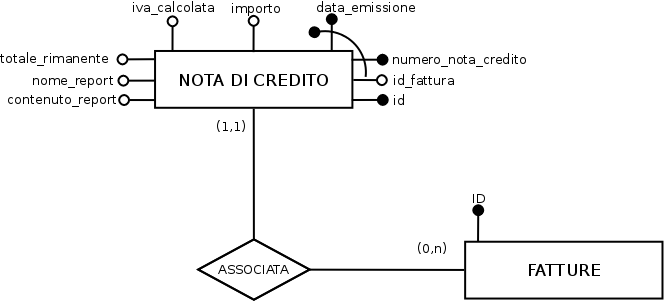
\includegraphics[scale=0.5]{img/schema_concettuale}
\newline
Sono state attuate le seguenti scelte sugli attributi:
\begin{enumerate}
    \item L' attributo \texttt{totale\_rimanente} anche se attributo 
        derivato viene comunque messo per velocizzare le operazioni di 
        visualizzazione delle fatture in modo che non si debba fare ogni volta 
        i calcoli dell’ imponibile con le note di credito.
    \item Sono presenti due chiavi, la prima, chiave primaria, è un \texttt{id} 
        numerico auto incrementante mentre la seconda, chiave canditata, è 
        data dalla coppia \texttt{numero\_nota\_credito} e 
        \texttt{data\_emissione}.
        L'attributo \texttt{id\_fattura} è una chiave esterna ed è associata 
        con l'attributo \texttt{id} che è chiave dell' entità fattura.
    \item Abbiamo due attributi, \texttt{nome\_report} e 
        \texttt{contenuto\_report}, che contegono il nome e il contenuto 
        del file \texttt{.pdf} della nota di credito appena generata.
    \item Sono stati inseriti inoltre solo l’importo e l’ IVA calcolata in 
        quanto la percentuale dell’ IVA utilizzata e l’importo totale della 
        nota di credito possono essere ricavate dagli attributi importo e 
        IVA calcolata.
\end{enumerate}
\subsection{Schema Logico}
Si è quindi passato poi allo schema logico ricavato da quello concettuale.
\newline
\newline
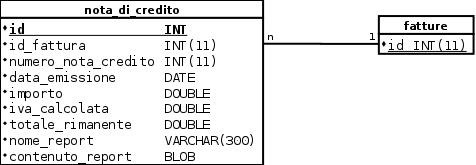
\includegraphics[scale=0.5]{img/schema_logico}
\newline
Come numero di cifre intere è stato scelto undici per rimanere in linea con il
numero di cifre dell' id della tabella \texttt{fattura}
\subsection{Implementazione Fisica}
Il codice della tabella in SQL è il seguente
\lstinputlisting[basicstyle=\ttfamily\scriptsize,title=Codice SQL della tabella]{code/tabella.sql}
Per tutti i campi è stato deciso di renderli tutti non nulli perché alla
generazione della nota di credito tutti i campi devono essere compilati.
\section{Implementazione dell' applicativo.}
Si è passati poi alla scrittura del codice per integrare la nuova funzionalità
nell' applicativo.
Per questa parte sono stato aiutato da due sviluppatori interni all' azienda
di nome Mauro Veronese della sede di Padova e Rocco Spenza della sede di Roma.
\subsection{Bean delle note di credito}
Come prima cosa dopo la creazione del database si è dovuto scrivere il Bean per 
poter mappare la tabella in Hibernate.
\lstinputlisting[basicstyle=\ttfamily\scriptsize,firstline=22,lastline=64,title=Bean della tabella delle note di credito]{code/bean/NotaDiCredito.java}
Si è scelto inoltre di indicare tramite le notazioni Java di effettuare un Join
automatico con la tabella delle fatture essendo che nella maggioranza delle 
operazioni era necessario avere anche i dati della fattura associata.
\subsection{Lista delle fatture}
Successivamente si è passato a modificare la lista di visualizzazione delle 
fatture fatta precedentemente 
integrando l' inserimento delle note di credito all' interno dell' interfaccia 
di inserimento fatture.
\newline
\newline
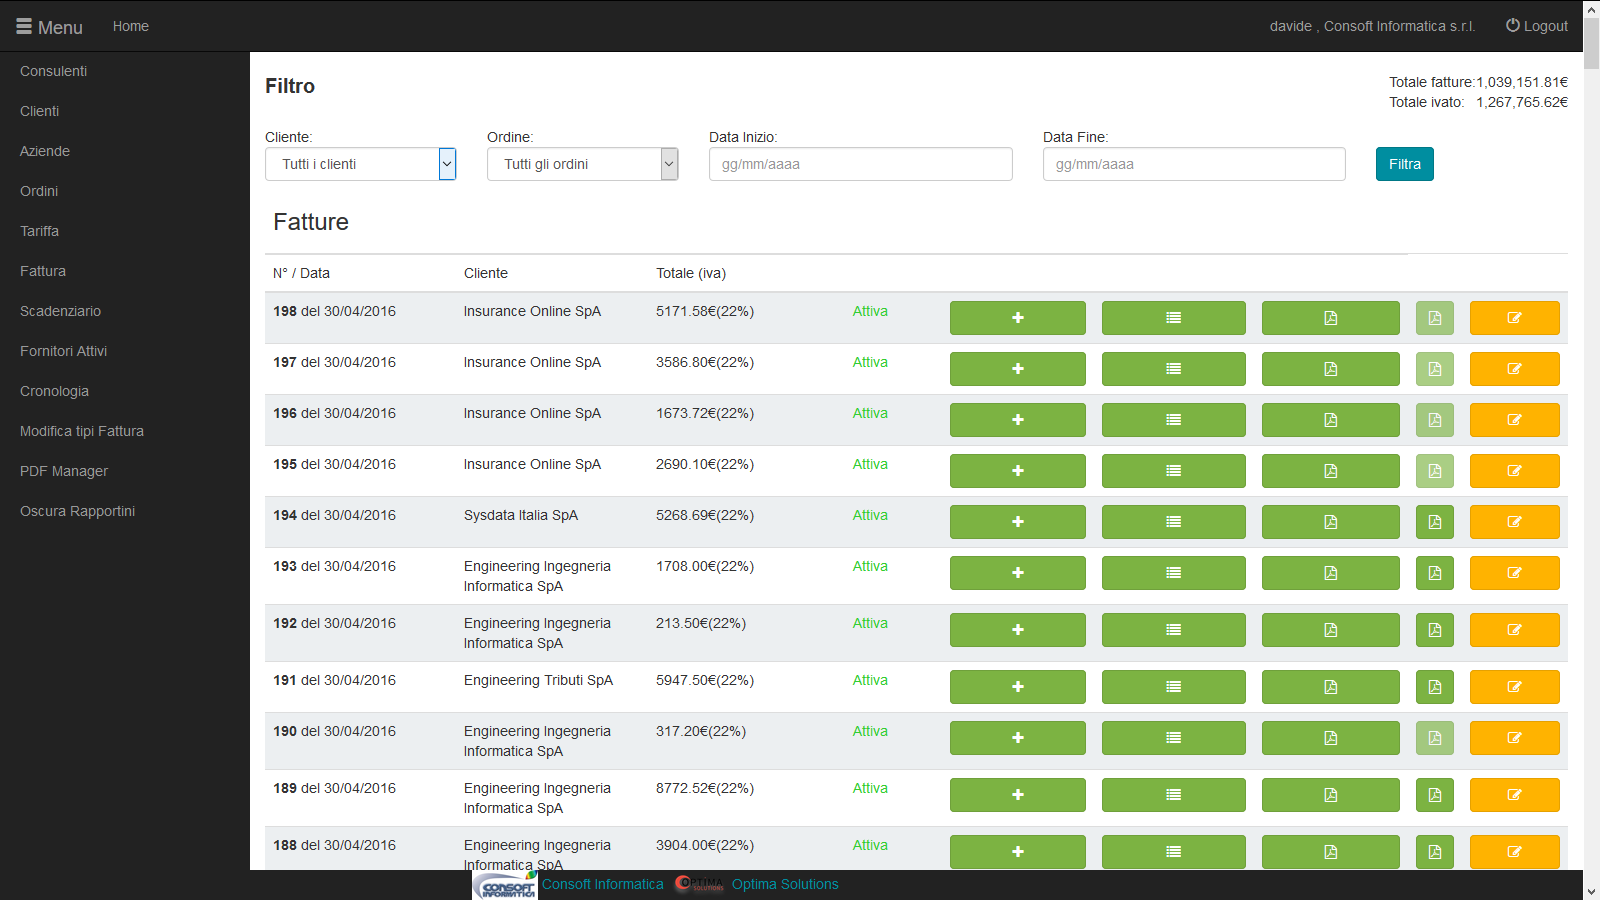
\includegraphics[scale=0.4]{img/lista_fatture}
\newline
Sono stati inseriti i due bottoni verdi \includegraphics[scale=0.4]{img/add} e 
\includegraphics[scale=0.4]{img/list} i quali sono rispettivamente per l' inserimento e 
la visualizzazione della nota di credito per ogni fattura.
\subsection{Inserimento e modifica della nota di credito}
Si è passato poi alla scrittura dell' interfaccia di inserimento e modifica
della nota di credito che possiamo vedere nell' immagine sottostante.
\newline
\newline
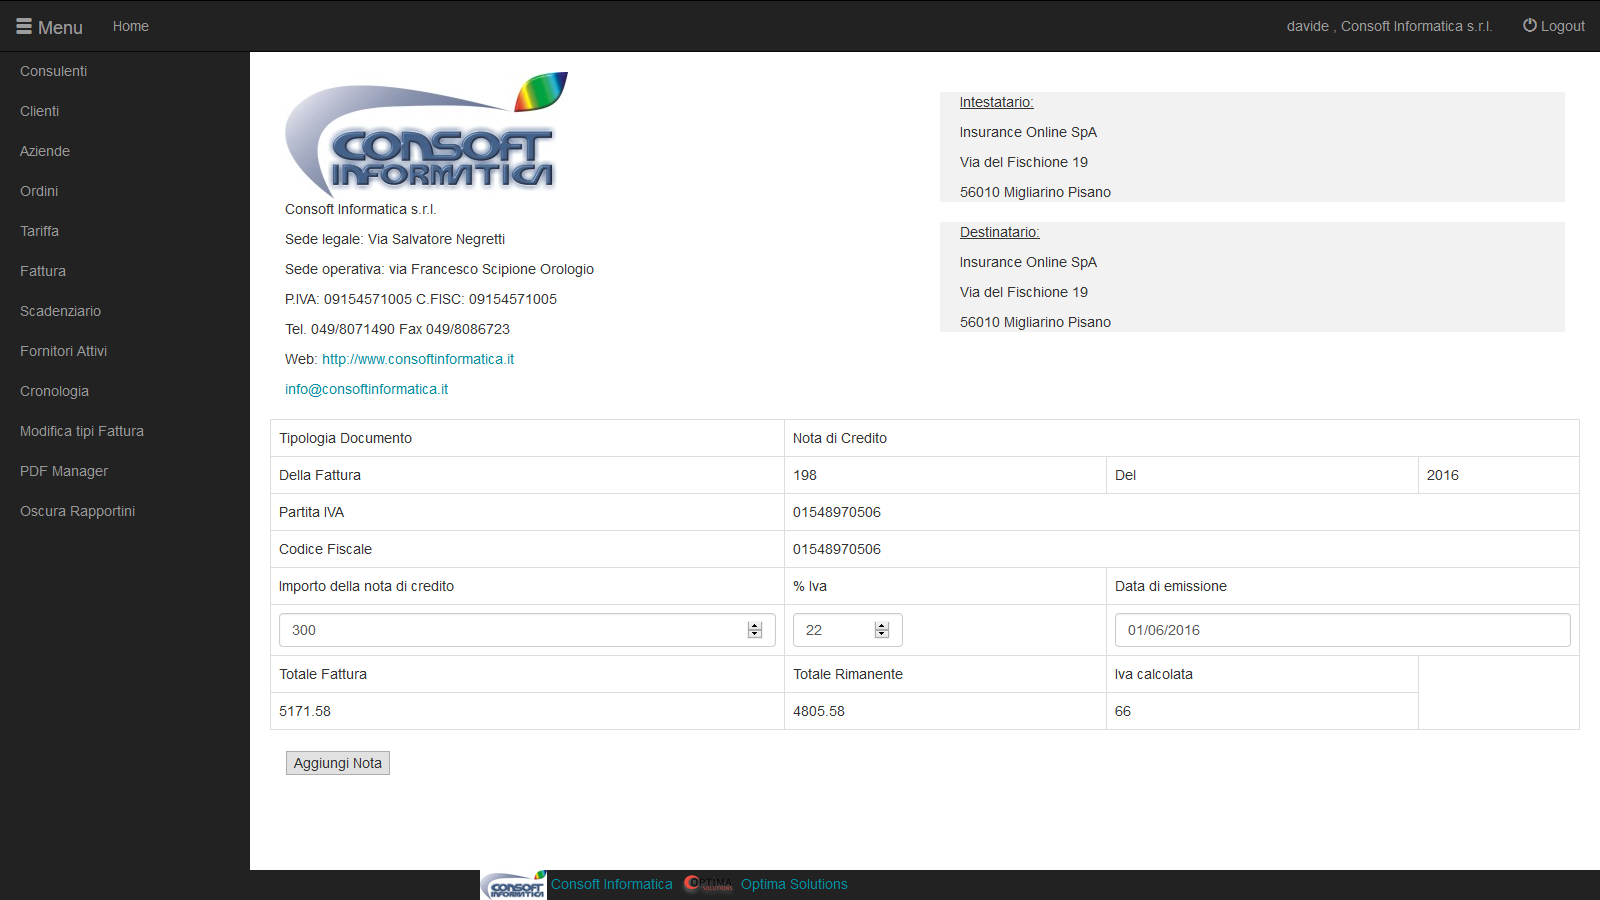
\includegraphics[scale=0.4]{img/inserimento_nota_credito}
\newline
La cui struttura è data dal seguente codice html.
\lstinputlisting[firstline=100,lastline=172,basicstyle=\ttfamily\scriptsize,title=Codice Html della parte frontend]{code/view/inserimentoModificaNoteCredito.jsp}
Dove \(\texttt{\$\{azione\}}\) indica il tipo di web request che deve essere
fatta alla sottomissione della form.
La variabile \texttt{azione} viene determinata attraverso questo codice 
presente nella pagina jsp.
\lstinputlisting[firstline=8,lastline=14,basicstyle=\ttfamily\scriptsize,title=Codice per la decisione dell' azione da compiere]{code/view/inserimentoModificaNoteCredito.jsp}
Questo perché la stessa pagina viene utilizzata sia per la fase di modifica sia
in quella di inserimento di una nuova nota di credito.
Il calcolo del totale che verrà detratto in front end viene fatto al momento 
grazie a codice \texttt{Javascript/jQuery} che esegue i calcoli ogni 
volta che l'importo o l' iva viene modificato come si può vedere nel 
codice sottostante.
\lstinputlisting[firstline=175,lastline=190,basicstyle=\ttfamily\scriptsize,title=Codice javascript per la parte frontend]{code/view/inserimentoModificaNoteCredito.jsp}
Tutti i calcoli però vengono fatti nuovamente tramite Java dentro al controller
per evitare manomissioni nell' inserimento semplicemente modificando 
l'\texttt{html}.
Come prima cosa all' interno della form abbiamo specificato una classe che 
serve per validare i dati inseriti.
\lstinputlisting[firstline=16,lastline=33,basicstyle=\ttfamily\scriptsize,title=form di controllo delle note di credito]{code/form/NotaCreditoForm.java}
Il cui oggetto viene specificato nell' attributo \texttt{modelAttribute} del 
form.
\lstinputlisting[firstline=257,lastline=293,basicstyle=\ttfamily\scriptsize,title=parte di reperimento dati e controllo del controller delle note di credito]{code/controller/NotaCreditoController.java}
Infine, se tutti i controlli vanno a buon fine, avviene la creazione della nota di 
credito in formato \texttt{pdf} e il caricamento di tutti i dati nel database
come mostrato nel codice sottostante.
\clearpage
\lstinputlisting[firstline=342,lastline=375,basicstyle=\ttfamily\scriptsize,title=generazione del pdf e caricamento di tutti i dati]{code/controller/NotaCreditoController.java}
\subsection{Lista delle note di credito}
La lista delle note di credito relativa ad una fattura può essere visualizzata
in due modi
\begin{enumerate}
    \item Attraverso la pressione del tasto
         nella lista delle fatture.
    \item Appena finito di compilare e salvare nel database una nota di credito.
\end{enumerate}
\subsubsection{Front End}
Un esempio di lista delle note di credito è la seguente
\newline
\newline
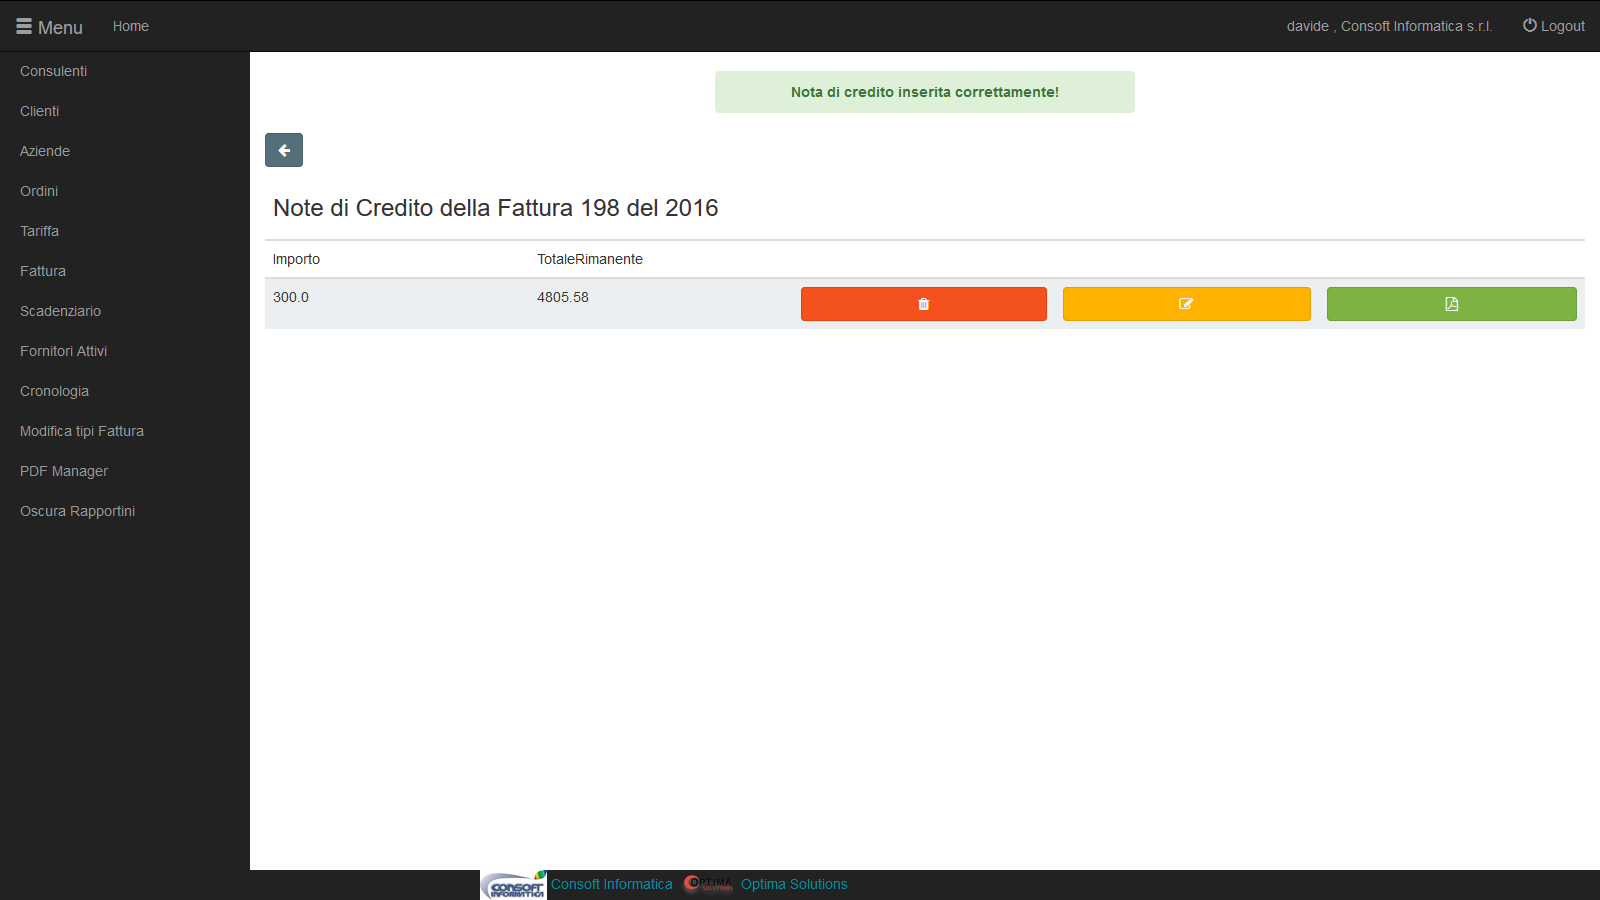
\includegraphics[scale=0.4]{img/visualizzazione_note_credito}
\newline
\begin{thebibliography}{9}
    \bibitem{consoft:descrizione} Sito ufficiale Consoft Informatica \newline
    \texttt{http://www.consoftinformatica.it}
    \bibitem{apress:introducing_spring_framework}Felipe Gutierrez, 
    \emph{Introducing Spring Framework: A Primer}, Apress.
    \newline
\end{thebibliography}
\end{document}
